\documentclass{article}
\usepackage[utf8]{inputenc}

\usepackage{natbib}
\usepackage{amsthm}
\usepackage{amssymb}
\usepackage{float}
\usepackage{algorithm}
%\usepackage{algorithmic}
\usepackage{listings}
\lstset{
  basicstyle=\ttfamily,
  columns=fullflexible,
  frame=single,
  breaklines=true,
  tabsize=2
  %postbreak=\mbox{\textcolor{red}{$\hookrightarrow$}\space},
}
\usepackage{algpseudocode}

\usepackage{amsmath}%
\usepackage{MnSymbol}%
\usepackage{wasysym}%
\usepackage{graphicx}
\usepackage{csquotes}
\usepackage{geometry}
\geometry{
 a4paper,
 total={170mm,257mm},
 left=25mm,
 right=25mm,
 top=20mm,
 }

\begin{document}
\begin{titlepage}
\begin{center}


{\large Master 1 MoSIG}\\[0.5cm]
\vspace*{10cm}
{\Huge \textbf{Parallel Algorithms and Programming} }\\[0.5cm]
{\large Lab 2 report} \\[3cm]

% Author and supervisor
\noindent
\begin{minipage}{0.4\textwidth}

   \centering Member:\\Son-Tung DO

\end{minipage}%

\vfill
% Bottom of the page
{Grenoble, Mar 3, 2019}
\clearpage

%\tableofcontents

\end{center}
\end{titlepage}

\section{Exercise 1: Matrix Mutiplication}
We have the matrix multiplication have the parallel that has been scheduled differently. We observed that the order of the performance is as follows: Dynamic $>$ Runtime $>$ Guided $>$ Static.


Speeding up chart based on observation.
\begin{figure}[H]
	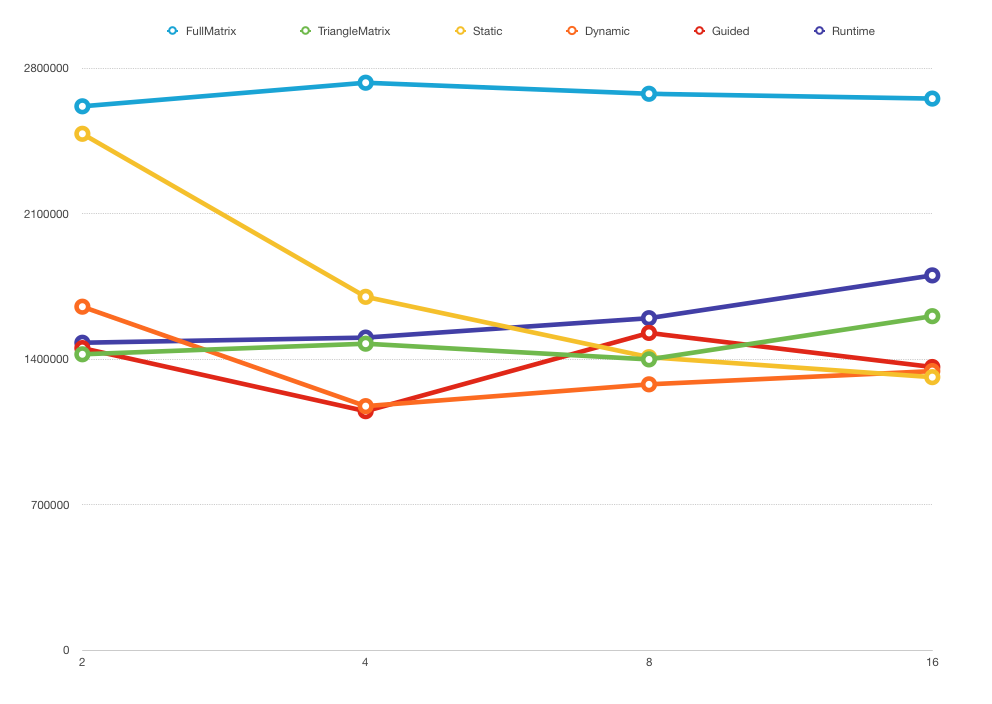
\includegraphics[width=\textwidth]{images/matrixChart.png}
	\caption{Speedup chart (cycles, threads)}
\end{figure}
\section{Exercise 2: Bubble Sort}
In Bubble sort parallel implementation, We make used of the reduction clause in the parralel of the inner loop to detect as if we have the 
\section{Exercise 3: Quick Sort}
\section{Exercise 4: Merge Sort}
We have the parallel implementation similar to sequential, but each time the recursive call is called, it create a task for threads to handle it.

Regarding the task's created with the size of the array, we will have $2^{n-1}$
\end{document}